\documentclass[10pt]{beamer}

\usepackage[UTF8]{ctex}
\usepackage{graphicx}
\usepackage{caption}
\usepackage{subcaption}
\usepackage{minted}
\usemintedstyle{manni}
\definecolor{bg}{rgb}{0.95,0.95,0.95}

\usepackage{float}

\usepackage{amsmath}

\usetheme{metropolis}
\usepackage{appendixnumberbeamer}

\usepackage{booktabs}
\usepackage[scale=2]{ccicons}

\usepackage{pgfplots}
\usepgfplotslibrary{dateplot}

\usepackage{xspace}
\newcommand{\themename}{\textbf{\textsc{metropolis}}\xspace}

\title{ID3}
\subtitle{算法实现及决策树可视化}
\date{\today}
\author{徐遥}
% \institute{None}
% \titlegraphic{\hfill\includegraphics[height=1.5cm]{logo.pdf}}

\begin{document}

\maketitle

\begin{frame}{目录}
  \setbeamertemplate{section in toc}[sections numbered]
  \tableofcontents[hideallsubsections]
\end{frame}

\section{可视化}

\begin{frame}[fragile]{Graphviz}

决策树的可视化利用了贝尔实验室开发的 \href{http://www.graphviz.org/}{Graphviz} 工具包。用户可以使用
DOT 语言来描述图形,然后利用该工具进行图形的布局与绘制,省去手动调整元素的大小与局部的繁琐过程。
对于决策树而言,我们只需要了解如何往有向图(digraph)添加节点与边。
\begin{figure}[!tbp]
  \begin{subfigure}[b]{0.48\textwidth}
    \inputminted[mathescape,breaklines,breakautoindent,fontsize=\tiny]{C}{./figures/graphviz_demo}
    \caption{DOT文件}
  \end{subfigure}
  \hfill
  \begin{subfigure}[b]{0.48\textwidth}
    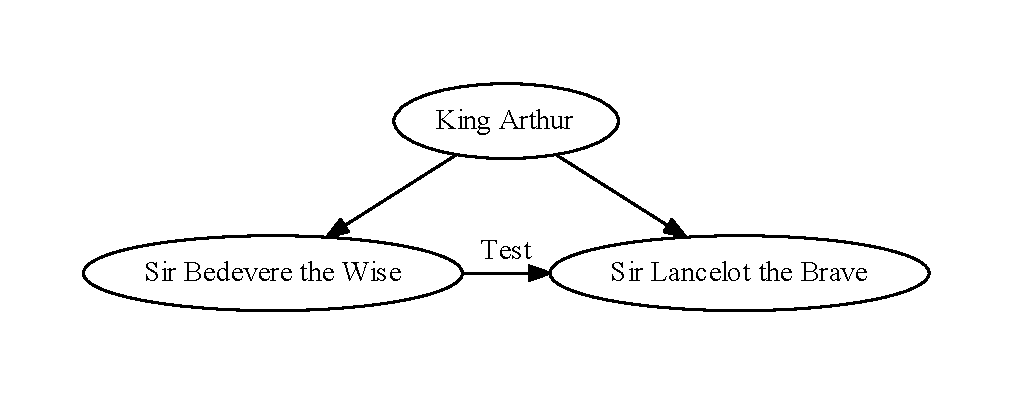
\includegraphics[width=\textwidth]{./figures/graphviz_demo.pdf}
    \caption{渲染后}
  \end{subfigure}
  \caption{Graphviz使用示例}\label{fig:dot_demo}
\end{figure}

\end{frame}

\begin{frame}[fragile]{Graphviz 的 Python 接口}
\mintinline{python}{graphviz} 提供了创建 DOT 文件的 Pyhton 接口。实际上,
图~\ref{fig:dot_demo} 就是其官方示例。
\inputminted[mathescape,linenos,frame=lines,framesep=2mm,breaklines,breakautoindent,fontsize=\small]{python}{./codes/graphviz_demo.py}
\end{frame}


\begin{frame}[fragile,allowframebreaks]{自动生成决策树的 DOT 文件}
有了上述工具,决策树的可视化就变得非常简单了:只需要递归地把所有节点和边加入有向图即可。
\begin{minted}[mathescape,linenos,frame=lines,framesep=2mm,breaklines,breakautoindent,fontsize=\small]{Python}
class ID3(object):
    class Node(object):
        @property
        def node_name(self):
            # 可视化时,每个node,必须要有独一无二的name
            return ''.join([self.attribute, str(self.id)])

        def add_to_graph(self, graph):
            graph.node(self.node_name, self.__str__())
            for edge_name, branch_node in self.branches.items():
                branch_node.add_to_graph(graph)
                graph.edge(self.node_name, branch_node.node_name, label=str(edge_name))

    def render_decision_tree(self, filename):
        if not self.root_node:
            raise ValueError('Tree not decided!')   
        from graphviz import Digraph
        dot_graph = Digraph(comment="Decision Tree")
        self.root_node.add_to_graph(dot_graph)
        dot_graph.render(filename)                    
\end{minted}
\end{frame}

\begin{frame}{生成树展示}
\begin{figure}[H]
  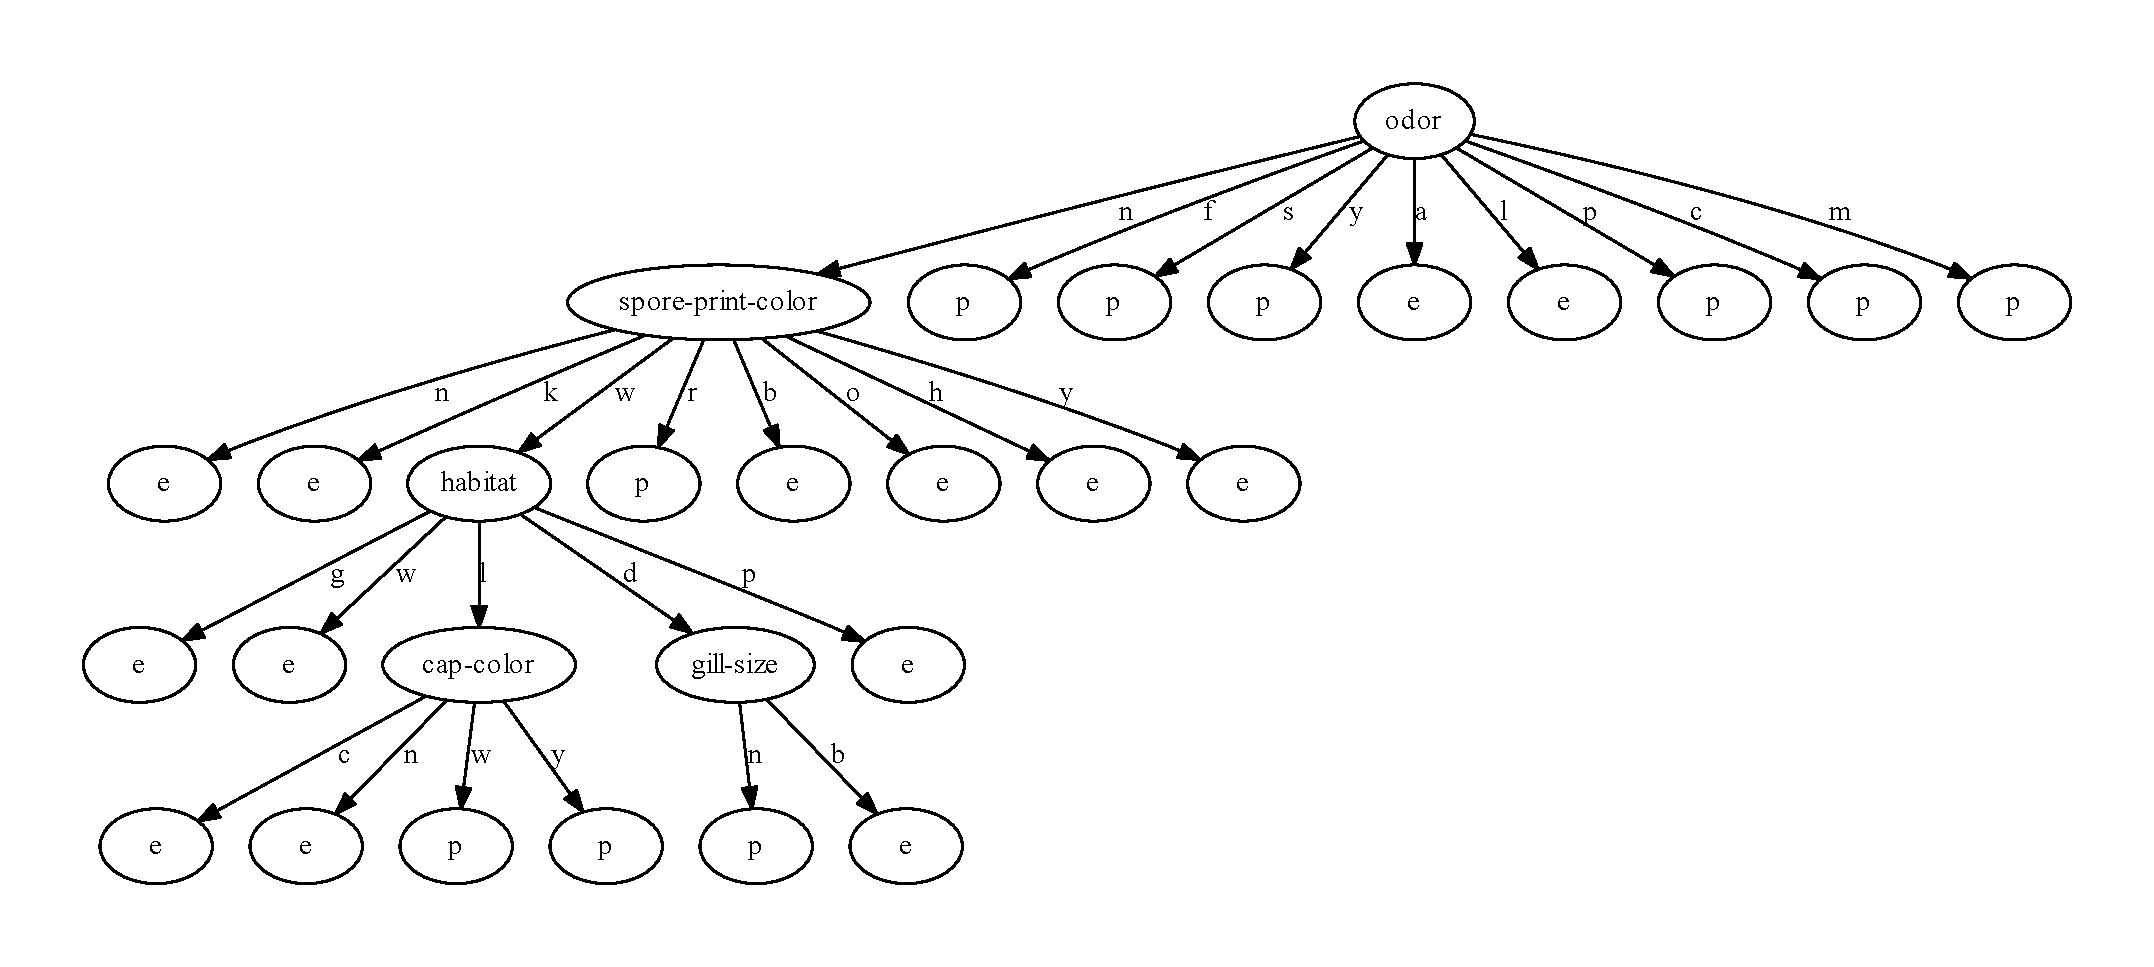
\includegraphics[width=\textwidth]{../mushroom_data/dtree.pdf}
  \caption{蘑菇毒性分类决策树}
\end{figure}            
\end{frame}


\end{document}
